\documentclass[a4paper,12pt]{article}

% --- LANGUAGE & FONT ---
\usepackage{vntex}
\usepackage[english]{babel}
\usepackage{amsmath, amssymb}

% --- PAGE & TEXT LAYOUT ---
\usepackage{a4wide}
\usepackage{geometry}
\geometry{a4paper, left=2cm, right=2cm, top=2.5cm, bottom=4.2cm, footskip=12mm}
\usepackage{setspace}
\usepackage{multicol}
\usepackage{enumitem}

% --- GRAPHICS & TABLES ---
\usepackage{graphicx}
\usepackage{epsfig}
\usepackage{svg}
\usepackage{tikz}
\usetikzlibrary{arrows,snakes,backgrounds,positioning,shapes,calc,fit}
\usepackage{booktabs}
\usepackage{multirow}
\usepackage{tabularx}
\usepackage{makecell}
\usepackage{array}
\usepackage[skip=5pt]{caption}
\usepackage{placeins}
\usepackage{float}       % added: the template uses [H]
\usepackage{longtable}   % added: long tables across pages

% --- COLOURS & CODE ---
\usepackage{color}
\usepackage{xcolor}
\usepackage{colortbl}    % added: coloured table rows
\usepackage{minted}
\usepackage{listings}
\usepackage{algorithm}
\usepackage{algpseudocode}
\usepackage[framemethod=tikz]{mdframed}

% --- HEADER & FOOTER ---
\usepackage{fancyhdr}
\usepackage{lastpage}

% --- HYPERREF (always load last) ---
\usepackage{hyperref}
\hypersetup{urlcolor=blue,linkcolor=black,citecolor=black,colorlinks=true}

% ================= COLOURS =================
\setlength{\columnseprule}{1pt}
\def\columnseprulecolor{\color{black}}
\definecolor{p1}{RGB}{52,101,164}
\definecolor{p2}{RGB}{78,154,6}
\definecolor{p3}{RGB}{204,0,0}
\definecolor{p4}{RGB}{117,80,123}
\definecolor{p5}{RGB}{193,125,17}
\definecolor{p6}{RGB}{32,128,128}
\definecolor{p7}{RGB}{90,90,90}
\definecolor{p8}{RGB}{170,60,120}

% ================= HEADER/FOOTER =================
\everymath{\color{blue}}
\setlength{\headheight}{40pt}
\pagestyle{fancy}
\fancyhead{}
\fancyhead[L]{
 \begin{tabular}{rl}
    \begin{picture}(25,15)(0,0)
    \put(0,-8){
\includegraphics[width=8mm, height=8mm]{hcmut.png}}
   \end{picture}&
    \begin{tabular}{l}
        \textbf{\ttfamily Ho Chi Minh City University of Technology - VNU-HCM}\\
        \textbf{\ttfamily Faculty of Computer Science and Engineering}
    \end{tabular}
 \end{tabular}
}
\fancyhead[R]{}
\fancyfoot{}
\fancyfoot[L]{\scriptsize \ttfamily \textcolor{blue}{Builders Buildathon 2026 - P2 Shopping Sessions \\ Team HCMUT TMT, November 2026}}
\fancyfoot[R]{\scriptsize \ttfamily Page {\thepage}/\pageref{LastPage}}
\renewcommand{\headrulewidth}{0.3pt}
\renewcommand{\footrulewidth}{0.3pt}

\setcounter{secnumdepth}{4}
\setcounter{tocdepth}{3}

% ================= COLOURED BOXES =================
% \partbox{color}{title}{content}: short box, no page break
\newcommand{\partbox}[3]{%
\begin{mdframed}[nobreak=true,linecolor=#1,linewidth=1.2pt,topline=false,rightline=false,bottomline=false,leftmargin=0pt,rightmargin=0pt,innerleftmargin=10pt,backgroundcolor=#1!6]
\textbf{\color{#1}#2}\par\smallskip #3
\end{mdframed}}
% \longbox{color}{title}{content}: long box, may break across pages
\newcommand{\longbox}[3]{%
\begin{mdframed}[linecolor=#1,linewidth=1.2pt,topline=false,rightline=false,bottomline=false,leftmargin=0pt,rightmargin=0pt,innerleftmargin=10pt,backgroundcolor=#1!6]
\textbf{\color{#1}#2}\par\smallskip #3
\end{mdframed}}
% \metabox{color}{workload}{prerequisites}{foundation for}{people}
\newcommand{\metabox}[5]{%
\begin{mdframed}[nobreak=true,linecolor=#1,linewidth=1pt,leftmargin=0pt,rightmargin=0pt,backgroundcolor=#1!15]
\textbf{Workload:} #2\par
\textbf{Prerequisites:} #3\par
\textbf{Foundation for:} #4\par
\textbf{People:} #5
\end{mdframed}}

% ================= HELPER MACROS (added for this report) =================
% \trial{...}: trial-run figure, not an official result
\newcommand{\trial}[1]{\textcolor{p5}{\textbf{[trial run]}~#1}}
% \src{...}: source of a figure
\newcommand{\src}[1]{{\footnotesize\textcolor{p7}{(source: #1)}}}
\newcommand{\fn}[1]{\texttt{\detokenize{#1}}}
\newcolumntype{L}[1]{>{\raggedright\arraybackslash}p{#1}}
\newcolumntype{C}[1]{>{\centering\arraybackslash}p{#1}}
\newcolumntype{Y}{>{\raggedright\arraybackslash}X}
\setlist{itemsep=1pt,topsep=2pt}
\renewcommand{\arraystretch}{1.15}

\begin{document}

\begin{titlepage}
\begin{center}
\Large Vietnam National University Ho Chi Minh City \\
\Large Ho Chi Minh City University of Technology \\
\Large Faculty of Computer Science and Engineering
\end{center}

\vspace{1cm}
\begin{center}

\includegraphics[width=4cm]{hcmut.png}
\end{center}
\vspace{1cm}

\begin{center}
\begin{tabular}{c}
    \textbf{\Large BUILDERS BUILDATHON 2026} \\[0.2cm]
    \textbf{\Large (Problem 2)} \\
    ~~\\
    \hline
    \\
    \multicolumn{1}{l}{\textbf{{\Large Problem overview}}}\\
    \\
    \textbf{{\LARGE Databricks -- Shopping Sessions}}\\[0.2cm]
    {\large Click-stream pipeline $\rightarrow$ two daily Parquet tables}\\
    \\
    \hline
\end{tabular}
\end{center}

\vspace{0.5cm}

\begin{table}[h]
\centering
\begin{tabular}{rrl}
\hspace{2cm} & Track: & Databricks - Shopping Sessions \\
& Team: & HCMUT TMT\\
& Student: & Dang Minh Triet - 2510249 \\
& Deadline: & 23:00 Sunday 22/11/2026 (GMT+7) \\
\end{tabular}
\end{table}

\vfill
\begin{center}
{\footnotesize Ho Chi Minh City, November 2026}
\end{center}
\end{titlepage}

\thispagestyle{fancy}
\newpage
\tableofcontents
\newpage

\sloppy

\section{Overview}

\subsection{General information}
\begin{table}[H]
\centering\small
\begin{tabularx}{\textwidth}{L{4.0cm}Y}
\toprule
\textbf{Item} & \textbf{Details} \\
\midrule
Track & Databricks -- Shopping Sessions (sponsor Databricks, \$5{,}000 prize, 116 teams on the practice board at the time of the screenshot) \\
Problem & Clean an online shop's CSV logs (page views, add-to-carts, purchases, ad clicks), join each person's IDs, build sessions, credit each session to the ad click that brought the shopper in, count assisting campaigns from the week before, and write two daily Parquet tables: \fn{/output/user_daily/} and \fn{/output/campaign_daily/}. The rules are exact, so there is one right answer; a fast answer that is almost right scores nothing \\
Deadline & \textbf{23:00 Sunday 22/11/2026 (GMT+7)}. At the time of writing (Sat 21/11, around 11:10) about 36 hours remain \\
Submission limit & 2 per hour (submit panel at the time: ``2 of 2 left this hour''). Rejected submissions never change the best score \\
How to submit & Public GitHub repo, \fn{Dockerfile} at the root, plus a commit; repo at most 50 MB with no data (the dataset is mounted at run time) \\
Build & linux/amd64 image of at most 8 GB; the build has network access for up to 10 minutes; build time is never scored \\
Run & 8 vCPUs (Intel Xeon hyperthreads, AVX-512 available), 24 GB RAM, no swap, no network; \fn{/data} read-only; \fn{/output} + \fn{/scratch} at most 50 GB together; root read-only except \fn{/tmp} 64 MB; uid 1000; at most 4096 processes/threads; stdout at most 50 MB \\
Environment variables & \fn{DATA_DIR=/data}, \fn{OUTPUT_DIR=/output}, \fn{SCRATCH_DIR=/scratch}, \fn{HOME=/scratch}, \fn{NCPU=8}, \fn{MEM_GB=24} \\
\bottomrule
\end{tabularx}
\caption{General information for P2 \src{track page, rules.md, starter README}}
\end{table}

\subsection{Scoring and how it is graded}
P2 is \textbf{graded fully automatically}: correctness by exact comparison with the answer, then run time. There is no AI or human grading.

\begin{table}[H]
\centering\small
\begin{tabularx}{\textwidth}{L{3.3cm}YC{1.9cm}C{1.6cm}}
\toprule
\textbf{Step} & \textbf{Definition} & \textbf{Graded by} & \textbf{Part} \\
\midrule
Dev-set check & Each submission first runs on the public 1M-event dev set (at most 3 minutes). If it fails, you get the differing rows and your logs, and it stops & auto & 2.2--2.7 \\
Practice run & Timed once on hidden practice data (about 20 million events). Under 20 s it is timed 3 times and the median counts. Limit: at most 2$\times$ the baseline time and never over 5 minutes & auto & 2.8 \\
Correctness & A wrong table, a crash, or hitting the memory, disk, stdout or time limit stops the submission. Hidden runs only report the exit code, whether memory ran out, and counts of missing/extra/differing rows & auto & 2.7 \\
Score & Wall time from container start to exit (including engine start-up and reading CSVs), lower is better & auto & 2.8 \\
Final & The chosen commit is rebuilt and timed 3 times on about 60 million new events, each run capped at 3 minutes. Any run over 3 minutes means no final score; otherwise the median counts. At least the 10 fastest are retimed 7 times alone on an idle machine & auto & 2.8 \\
Ties & The earlier submission ranks first & auto & -- \\
\bottomrule
\end{tabularx}
\caption{P2 rubric \src{track page}}
\end{table}

\begin{table}[H]
\centering\small
\begin{tabular}{lrl}
\toprule
\textbf{Practice board (screenshot 21/11)} & \textbf{Time} & \textbf{Note} \\
\midrule
Rank 1 (Mahalas) & 0.68 s & \\
Rank 2 / 3 & 0.75 s / 0.79 s & \\
Rank 10 & 0.99 s & \\
Around rank 50 & 1.6 s & \\
Around rank 75 & 2.5 s & \\
Rank 100 & 8.00 s & \\
Baseline (PySpark starter, local mode) & 172.00 s & \\
Teams & 116 & \\
\bottomrule
\end{tabular}
\caption{Practice leaderboard snapshot. The page says practice times can vary by up to about 20\% across scoring machines, so small gaps are not meaningful}
\end{table}

\begin{mdframed}[linecolor=orange,linewidth=1pt,backgroundcolor=orange!8]
\textbf{Two survival conditions:} (1) \emph{exact correctness}, otherwise there is no score at all; (2) the final uses about 3 times the practice data and cuts off at 3 minutes, so the page advises \textbf{staying under about 60 s in practice}. Most teams on the board are already under 3 s, so a good rank also needs speed.
\end{mdframed}

\subsection{Sources and conventions for figures}
\begin{itemize}
  \item \textbf{Primary sources:} the track page (screenshot) and \fn{rules.md}. The page says that where a starter and \fn{rules.md} disagree, \fn{rules.md} wins. The repo has no forum Q\&A yet.
  \item \textbf{For reference:} the 3 starters (PySpark, DuckDB, Polars; identical 36 fixtures), \fn{generator/} (Rust source), \fn{dev-answer/}.
  \item Figures marked \trial{} come from my runs on a 2-vCPU trial machine, \emph{not official results}.
\end{itemize}

\begin{table}[H]
\centering\small
\begin{tabularx}{\textwidth}{L{5.2cm}Y}
\toprule
\textbf{Dev set (seed 1)} & \textbf{Value} \\
\midrule
Command & \fn{generate --seed 1 --events 1000000 --clicks 250000 --output dev} \\
\trial{Generation time} & 0.47 s (after \fn{cargo build --release} took 2.4 s) \\
\trial{Size, files} & 92 MB; 30 event files (79 MB), 40 click files (12 MB), 14 link files (940 KB) \\
\trial{Data rows (excluding headers)} & events 1,072,086; clicks 255,240; links 44,874; \fn{products.csv} 50,000; \fn{campaigns.csv} 2,000 \\
Time window & 2027-12-09T00:00:00Z to 2027-12-23T00:00:00Z \\
Dev answer (\fn{dev-answer/}) & \fn{user_daily.csv} 117,038 rows; \fn{campaign_daily.csv} 27,400 rows \\
\bottomrule
\end{tabularx}
\caption{The 1M-event dev set \src{generator, dev-answer.zip}}
\end{table}

\subsection{Dependency diagram}
\begin{center}
\begin{tikzpicture}[
  box/.style={draw,rounded corners,thick,text width=3.0cm,minimum height=1.1cm,align=center,font=\small},
  ext/.style={draw,dashed,rounded corners,text width=3.6cm,minimum height=1cm,align=center,font=\small,fill=gray!8},
  arr/.style={->,thick,>=stealth},
  lab/.style={font=\scriptsize,fill=white,inner sep=1pt}]
  \node[ext] (c) at (0,2.4) {\textbf{Shared}: public repo, Docker (shared with P1, P4)};
  \node[box,draw=p1,fill=p1!10] (a) at (0,0) {\textbf{2.1} Engine choice, repo setup};
  \node[box,draw=p2,fill=p2!10] (b) at (4.3,0) {\textbf{2.2} CSV reading per the dialect};
  \node[box,draw=p3,fill=p3!10] (d) at (8.6,1.2) {\textbf{2.3} Timestamps, validation};
  \node[box,draw=p4,fill=p4!10] (e) at (8.6,-1.2) {\textbf{2.4} Linked IDs};
  \node[box,draw=p5,fill=p5!10] (f) at (12.9,1.2) {\textbf{2.5} Events $\rightarrow$ sessions};
  \node[box,draw=p6,fill=p6!10] (g) at (12.9,-1.2) {\textbf{2.6} Clicks: credit, assists};
  \node[box,draw=p7,fill=p7!10] (h) at (8.6,-3.6) {\textbf{2.7} Parquet output, testing};
  \node[box,draw=p8,fill=p8!10] (i) at (2.6,-3.6) {\textbf{2.8} Speed optimisation};
  \draw[arr] (c) -- (a);
  \draw[arr] (a) -- (b);
  \draw[arr] (b) -- (d);
  \draw[arr] (b) -- (e);
  \draw[arr] (d) -- (f);
  \draw[arr] (e) -- (f);
  \draw[arr] (e) -- (g);
  \draw[arr] (f) -- node[lab,right=2pt]{session start} (g);
  \draw[arr] (g) |- (h);
  \draw[arr] (h) -- node[lab,above=2pt]{correct first, then fast} (i);
\end{tikzpicture}
\end{center}
P2 does not depend on the results of P1, P3 or P4; it only shares infrastructure (public repo, Docker linux/amd64) and the time budget.

\subsection{Repo status}

\begin{table}[H]
\centering\small
\begin{tabularx}{\textwidth}{L{4.2cm}Y}
\toprule
\textbf{Item} & \textbf{Status (read on 21/11, around 11:10)} \\
\midrule
Main repo & \fn{martin-danggg/HCMUT_TMT_Builders_BUILDATHON}, branch \fn{main}, remote \fn{origin} over SSH \\
Latest commit & \fn{55687de} ``Initial commit'', 21/11/2026 10:41:21 +0700, author Triet Dang. This is the only commit \\
Committed files & Only \fn{README.md} (31 bytes, a one-line title) \\
Not committed (untracked) & \fn{p1_Builders/} (2.9 MB), \fn{p2_Databricks/} (5.7 MB), \fn{p3_Machina/} (48 KB), \fn{p4_RWX/} (404 KB): all of it is starter files from the organisers; no solution code yet \\
\fn{reports/} folder & Holds this overview (Vietnamese and English, not committed) \\
Main repo \fn{.gitignore} & Ignores the 3 \fn{submission/} folders (separate repos) and \fn{p3_Machina/work/} (P3 data must stay private) \\
Separate submission repos (created on GitHub, public) & P1: \fn{martin-danggg/hcmut-tmt-p1-mech-royale} $\rightarrow$ \fn{p1_Builders/submission/}\allowbreak\fn{hcmut-tmt-p1-mech-royale/} (commit \fn{f4e1861})\newline P2: \fn{martin-danggg/hcmut-tmt-p2-shopping-sessions} $\rightarrow$ \fn{p2_Databricks/submission/}\allowbreak\fn{hcmut-tmt-p2-shopping-sessions/} (commit \fn{21cd7e4})\newline P4: \fn{martin-danggg/hcmut-tmt-p4-blast-radius} $\rightarrow$ \fn{p4_RWX/submission/}\allowbreak\fn{hcmut-tmt-p4-blast-radius/} (commit \fn{2a682dc})\newline The starter skeleton is cloned, committed as ``Setup: add requirements'' and pushed to \fn{main} by \fn{tools/setup_submissions.sh} \\
\bottomrule
\end{tabularx}
\caption{Status of the main repo, shared by all 4 problems}
\end{table}

\begin{mdframed}[linecolor=orange,linewidth=1pt,backgroundcolor=orange!8]
\textbf{Submitting through separate repos (decided):} P1, P2 and P4 all require \emph{a public GitHub repository with the \fn{Dockerfile} at the root} of the submitted commit. The main repo is a monorepo (p1--p4 in subfolders), so \textbf{the main repo is never submitted}. Each track has its own public repo, kept locally in \fn{pX_.../submission/hcmut-tmt-pX-.../}; each of those folders is an independent git repo with its own remote, and the main repo ignores them via \fn{.gitignore}. To submit: paste the track repo's link (e.g. \fn{https://github.com/martin-danggg/hcmut-tmt-p4-blast-radius}) into \emph{Public GitHub repository}; leave \emph{Commit} empty to use the newest commit on \fn{main}. Keep the repo public, with every submitted commit, until results are published. P3 needs no GitHub (it is submitted through the team's \fn{gs://} folder).
\end{mdframed}


\begin{table}[H]
\centering\small
\begin{tabularx}{\textwidth}{L{5.3cm}C{1.9cm}Y}
\toprule
\textbf{P2 component} & \textbf{Present?} & \textbf{Note} \\
\midrule
\fn{rules.md} & Yes & Full specification (17 KB) \\
DuckDB / Polars / PySpark starters (.zip + unpacked) & Yes & Empty pipelines that only write the right schema; duckdb 1.5.6, polars 2.1.0, pyspark 4.0.1; Python 3.12-slim-bookworm \\
36 fixtures (\fn{A1}--\fn{A12}, \fn{E1}--\fn{E20}, \fn{L1}--\fn{L4}) & Yes & Identical in all 3 starters; expected rows written by hand from the rules \\
\fn{generator/} (Rust) and \fn{dev-answer/} & Yes & Needs Rust $\ge$ 1.85 to build \\
The 1M-event dev set (\fn{dev/}) & No & Not for the submission repo; generated with the generator (I generated one outside the repo as a trial) \\
Separate submission repo \fn{hcmut-tmt-p2-}\allowbreak\fn{shopping-sessions} & Yes & \fn{p2_Databricks/submission/}\allowbreak\fn{hcmut-tmt-p2-shopping-sessions/}: the whole \fn{starter-duckdb} (Dockerfile, Makefile, empty pipeline, scripts, 36 fixtures), \fn{TEAM.md} filled in, \fn{.gitignore} blocking data; commit ``Setup: add requirements'' (\fn{21cd7e4}), then \fn{93d927b} ``Fix: keep CRLF in fixtures'': adds \fn{.gitattributes} (\fn{* -text}) because Git on Windows had turned the deliberate CRLF line of fixture E20 into LF \\
Team pipeline & No & Output of 2.1--2.8 \\
\bottomrule
\end{tabularx}
\caption{What P2 already has and what is missing}
\end{table}

\subsection{Assignments and schedule}
Working alone, so the ``reviewer'' column does not apply. Instead of review: 36/36 fixtures + \fn{check-dev} MATCH + the totals self-check (section 2.7) before every submission.

\begin{table}[H]
\centering\small
\begin{tabularx}{\textwidth}{C{1cm}L{2.6cm}YC{1.6cm}}
\toprule
\textbf{Part} & \textbf{Owner} & \textbf{Task} & \textbf{Review} \\
\midrule
2.1 & Dang Minh Triet & Pick the engine, create the submission repo from a starter & -- \\
2.2 & Dang Minh Triet & CSV reader that follows the \fn{rules.md} dialect & -- \\
2.3 & Dang Minh Triet & Convert the 3 timestamp forms, check windows and prices & -- \\
2.4 & Dang Minh Triet & Union-find over \fn{links/}, naming people & -- \\
2.5 & Dang Minh Triet & Dedup, filter, sessionize, day, categories & -- \\
2.6 & Dang Minh Triet & Click dedup, session credit, assists & -- \\
2.7 & Dang Minh Triet & Write Parquet, run fixtures, \fn{check-dev} & -- \\
2.8 & Dang Minh Triet & Measure and optimise run time & -- \\
\bottomrule
\end{tabularx}
\caption{P2 assignments}
\end{table}

There are no ``weeks'' or ``tag deadlines'': the only deadline is 23:00 Sunday 22/11. Suggestion: tag the locked commit \fn{p2-final}. P2 gets 6.5 hours out of about 25 working hours (26\%).

\begin{center}\small
\begin{longtable}{L{1.8cm}L{2.1cm}C{1.3cm}L{10.1cm}}
\toprule \textbf{Day} & \textbf{Time} & \textbf{Track} & \textbf{Task} \\ \midrule\endhead
Sat 21/11 & 11:15--12:00 & Shared & Create 3 separate public repos for P1, P2, P4 (Dockerfile at the root); check Docker/WSL2; P3: fetch the manifest, run \fn{get-input.sh --limit 100} \\
 & 12:00--15:30 & P4 & 4.1 environment + 4.2 coverage map at the pinned commit; 4.3--4.4 selector v1; \fn{make sample}; first submission \\
 & 15:30--18:00 & P1 & 1.1 infrastructure + 1.2 map + 1.3 movement/zone; submit bot v1 \\
 & 18:00--19:00 & -- & Break \\
\rowcolor{p2!15} & 19:00--22:30 & P2 & 2.1--2.7 correct version: 36/36 fixtures, \fn{check-dev} MATCH; first submission \\
 & 22:30--23:30 & P3 & 3.1 survey 100 sample files; start the full corpus download in the background overnight \\
 & 23:30--00:30 & P1 & 1.4 combat v2; submit (scored while sleeping) \\
Sun 22/11 & 00:30--07:30 & -- & Sleep (P3 download keeps running) \\
 & 07:30--10:30 & P3 & 3.2--3.5 pipeline v1 on the corpus; upload attempt 1 \\
\rowcolor{p2!15} & 10:30--12:30 & P2 & 2.8 speed optimisation; submit twice \\
 & 12:30--13:30 & -- & Lunch \\
 & 13:30--15:00 & P4 & 4.5 safety rules + worker-split tuning; submit \\
 & 15:00--18:00 & P1 & 1.5 loot/upgrades + 1.6 A/B loop (about 10 submissions) \\
 & 18:00--20:30 & P3 & 3.6 attempts 2--3 based on per-category scores \\
\rowcolor{p2!15} & 20:30--21:30 & P2 & Final improvements, submit \\
 & 21:30--22:00 & P4 & Final improvements, submit \\
 & 22:00--22:45 & Shared & Lock in: pick the final submission for each track, keep repos public, tag \fn{pX-final} \\
 & 22:45--23:00 & -- & Buffer. All tracks close at 23:00 \\
\bottomrule
\caption{Proposed schedule for all 4 tracks up to the 23:00 Sunday 22/11 deadline (highlighted rows are P2)}
\end{longtable}
\end{center}


\subsection{Choosing the overall approach}
\begin{table}[H]
\centering\small
\begin{tabularx}{\textwidth}{L{2.6cm}YYC{1.7cm}}
\toprule
\textbf{Engine} & \textbf{Pros} & \textbf{Cons} & \textbf{Chosen?} \\
\midrule
PySpark (starter) & JVM workarounds ready & Baseline 172 s; slow JVM start-up; easily over 3 minutes in the final & No \\
\textbf{DuckDB} & Compact SQL; very fast parallel CSV reads; ASOF JOIN, windows, range joins; spills to disk when RAM runs short & Its CSV reader does not match the dialect (reads \fn{""} as an empty string, repairs malformed lines), so whole lines must be read and split by hand & \textbf{Yes (v1)} \\
Polars & Fast, lazy/streaming & Also needs manual line splitting; Rust's regex \texttt{\textbackslash d} matches Unicode digits & Backup \\
Hand-written Rust & Fastest (top teams under 1 s); byte-level control & Slow to write and easy to get wrong with 36 hours left and 3 other tracks & v2 if time allows \\
Plain Python & Easy to get right & Slow (tens of millions of lines) & No \\
\bottomrule
\end{tabularx}
\caption{Engine comparison for P2}
\end{table}

\textbf{Choose DuckDB for the first correct version}, because: (1) correctness is a hard requirement, and SQL lets each rule be written as a separately testable step; (2) reading whole lines and splitting them in SQL keeps full control over the dialect while still reading in parallel; \trial{reading the 1.07 million event lines (81 MB) raw takes 0.10 s, splitting into 7 fields 0.11 s, on 2 vCPUs}; (3) the ID graph is handled in Python/scipy rather than recursive SQL. If the DuckDB version is correct and time remains, rewrite the hot path in Rust, using the DuckDB version as the reference.

\newpage
\section{Parts of the work}

% ---------------------------------------------------------------
\subsection{2.1 Engine choice and repo setup}
\partbox{p1}{1. What the task requires}{A public repo with the \fn{Dockerfile} at the root; \fn{CMD} runs with no arguments, and exit code 0 means ``done, check my output''. Write nothing outside \fn{/output} and \fn{/scratch}; no network at run time.}
\partbox{p1}{2. Goal when done}{Repo \fn{hcmut-tmt-p2-}\allowbreak\fn{shopping-sessions} (created) built from \fn{starter-duckdb}; \fn{make build} and \fn{make fixtures} run (even if still wrong); \fn{generate} on the PATH and a \fn{dev/} folder for testing.}
\partbox{p1}{3. Input data and prerequisite knowledge}{
\textbf{Data:} \fn{starter-duckdb/}, \fn{generator/}.\\
\textbf{Knowledge:} Docker buildx, how the starter runs with the scorer's flags (\fn{scripts/docker_run.sh}), a Rust toolchain to build the generator.}
\partbox{p1}{4. Files to build on $\rightarrow$ files to produce}{
\textbf{Build on:} \texttt{starter-duckdb/\{Dockerfile, Makefile, run.sh, requirements.txt, pipeline/pipeline.py, scripts/*, fixtures/*\}}.\\
\textbf{Produce:} a submission repo laid out like the starter, with \fn{TEAM.md} filled in.}
\longbox{p1}{5. Approach and concrete steps}{
\begin{enumerate}[leftmargin=1.4em]
  \item Create a public repo and copy the contents of \fn{starter-duckdb/} to its root (the fixtures come along since they live in the starter folder).
  \item \fn{cargo build --release} in \fn{generator/}, copy \fn{target/release/generate} onto the PATH; \fn{make dev}; unzip \fn{dev-answer.zip} into \fn{dev-answer/}.
  \item No Docker needed for fast iteration: \fn{python3 scripts/run_fixtures.py fixtures -- python3 pipeline/pipeline.py} (the compare script needs \fn{pip install polars}).
  \item Add a \fn{.gitignore} for \fn{dev/}, \fn{out/}: the repo is limited to 50 MB and must contain no data.
\end{enumerate}}
\partbox{p1}{6. Special requirements and pitfalls}{The image must be linux/amd64 (Intel Xeon scorers). The process runs as uid 1000: every temp directory (DuckDB \fn{temp_directory}, \fn{TMPDIR}, \fn{HOME}) must point into \fn{/scratch}; the starter's \fn{run.sh} already does this.}
\metabox{p1}{5\% of P2 (1.3\% of all 4 problems), about 0.3 hours}{The ``Shared'' block (GitHub, Docker)}{2.2}{Skipped (working alone)}

% ---------------------------------------------------------------
\subsection{2.2 CSV reading per the dialect}
\partbox{p2}{1. What the task requires}{Comma-separated, UTF-8, only \texttt{\textbackslash n} ends a line (\texttt{\textbackslash r} is an ordinary character). Any field may be wrapped in double quotes; quotes are syntax, \fn{""} is an empty field; empty fields are null. Lines with the wrong field count, a quote anywhere except around a whole field, or empty lines are malformed and dropped. Spaces are part of the value. Every file has a header; read every \fn{*.csv} in \fn{events/}, \fn{clicks/}, \fn{links/} (some hold only the header).}
\partbox{p2}{2. Goal when done}{Three raw tables \fn{events_raw}, \fn{clicks_raw}, \fn{links_raw} with the right column counts, quotes removed, nulls in the right places, malformed lines dropped. Passes the dialect fixtures: E13, E15, E19, E20, L3.}
\partbox{p2}{3. Input data and prerequisite knowledge}{
\textbf{Data:} \fn{/data/events/*.csv} (7 columns), \fn{clicks/*.csv} (4 columns), \fn{links/*.csv} (2 columns).\\
\textbf{Knowledge:} DuckDB's \fn{read_csv} with \fn{delim}, \texttt{quote=\textquotesingle{}\textquotesingle{}}, \texttt{escape=\textquotesingle{}\textquotesingle{}}, \fn{header}, \texttt{new\_line=\textquotesingle{}\textbackslash n\textquotesingle{}}; string functions \fn{string_split}, \fn{regexp_matches} (use \fn{[0-9]}, not \texttt{\textbackslash d}).}
\partbox{p2}{4. Files to build on $\rightarrow$ files to produce}{
\textbf{Build on:} the ``CSV dialect'' section of \fn{rules.md}, \fn{fixtures/README.md}.\\
\textbf{Produce:} a \fn{read_table(glob, ncols)} function in \fn{pipeline/pipeline.py} (or \fn{pipeline/csv.sql}).}
\longbox{p2}{5. Approach and concrete steps}{
\textbf{Idea:} never let DuckDB interpret commas or quotes. Read each line as one string, then split it yourself.
\begin{enumerate}[leftmargin=1.4em]
  \item Read whole lines: \texttt{read\_csv(glob, columns=\{\textquotesingle{}line\textquotesingle{}:\textquotesingle{}VARCHAR\textquotesingle{}\}, delim=chr(1), quote=\textquotesingle{}\textquotesingle{}, escape=\textquotesingle{}\textquotesingle{}, header=true, auto\_detect=false, new\_line=\textquotesingle{}\textbackslash n\textquotesingle{})}. The header is skipped per file; a line equal to the header in the middle of a file is still data (fixture L3).
  \item Split: \texttt{f = string\_split(line, \textquotesingle{},\textquotesingle{})}; keep lines with \fn{len(f) = ncols}. An empty line gives 1 field, so it drops out automatically when \fn{ncols} $\ge$ 2.
  \item For each field: if it has no \fn{"}, keep it; if it has the form \fn{"..."} (quotes at both ends, none inside), strip them; otherwise the line is malformed. Empty fields (after stripping) become NULL.
  \item No trimming, no case changes; keep a trailing \texttt{\textbackslash r} on the last field so later steps reject it (price \texttt{1000\textbackslash r} is invalid, a \fn{ts} with \texttt{\textbackslash r} is invalid).
  \item Check each dialect fixture by printing the raw table and comparing with the description in \fn{fixtures/README.md}.
\end{enumerate}}
\partbox{p2}{6. Special requirements and pitfalls}{Fixture L3 has a quoted ID containing a tab (\texttt{"A\textbackslash tB"}) that becomes the name of the person made of \fn{u4} and \fn{u1}. The fake delimiter \fn{chr(1)} must not appear in the data (the rules do not strictly forbid it; read \fn{generator/src/text.rs} to be sure, or add a check). Malformed lines are about 0.05\% of lines.}
\metabox{p2}{15\% of P2 (3.9\% of total), about 1.0 hour}{2.1}{2.3, 2.4}{Skipped (working alone)}

% ---------------------------------------------------------------
\subsection{2.3 Timestamps and validation}
\partbox{p3}{1. What the task requires}{\fn{ts} comes in 3 forms: F1 \fn{YYYY-MM-DDTHH:MM:SSZ}; F2 with an offset \fn{+HH:MM}/\fn{-HH:MM} (hours 00--23, minutes 00--59, subtract it to get UTC); F3 digits only = epoch milliseconds (leading zeros allowed). Anything else is bad (fractional seconds, lowercase \fn{z}/\fn{t}, a space instead of \fn{T}, no zone, impossible dates, hour 24, second 60, an offset without a colon\ldots). Events need \fn{window_start <= ts < window_end}; clicks need \fn{window_start - 7 days <= ts < window_end}. \fn{ingest_ts} is always valid F1.}
\partbox{p3}{2. Goal when done}{A SQL \fn{parse_ts(s) -> BIGINT ms or NULL} and the validity conditions for events (type, product, price) and clicks (campaign). Passes E2, E7, E10, E12, E13, E17, E18, A10.}
\partbox{p3}{3. Input data and prerequisite knowledge}{
\textbf{Data:} raw tables from 2.2, \fn{manifest.json}, \fn{products.csv}, \fn{campaigns.csv}.\\
\textbf{Knowledge:} the Gregorian calendar (leap years: divisible by 4, except centuries not divisible by 400), converting dates to days since the epoch, int64 limits.}
\partbox{p3}{4. Files to build on $\rightarrow$ files to produce}{
\textbf{Build on:} the ``Timestamps'' section and the ``Validate'' steps for events and clicks in \fn{rules.md}.\\
\textbf{Produce:} macros \fn{parse_ts}, \fn{valid_price} in the pipeline.}
\longbox{p3}{5. Approach and concrete steps}{
\begin{enumerate}[leftmargin=1.4em]
  \item F1/F2: match a strict pattern, every digit being \texttt{[0-9]}:\\
  {\footnotesize\texttt{\textasciicircum[0-9]\{4\}-[0-9]\{2\}-[0-9]\{2\}T[0-9]\{2\}:[0-9]\{2\}:[0-9]\{2\}}\allowbreak\texttt{(Z|[+-][0-9]\{2\}:[0-9]\{2\})\$}}\\
  then slice out the numbers and check month 1--12, day $\le$ days in the month (with leap years), hour $\le$ 23, minute and second $\le$ 59, offset hour $\le$ 23, offset minute $\le$ 59.
  \item Convert to ms with arithmetic (days since epoch $\times$ 86,400,000 + ...) instead of \fn{strptime}, to be fast and avoid functions that silently ``fix'' bad dates. \fn{-00:00} is UTC.
  \item F3: \texttt{\textasciicircum[0-9]+\$}; strip leading zeros; more than 18 digits left means certainly outside the window (bad), so do not cast, avoiding overflow; otherwise cast to \fn{BIGINT}.
  \item Check windows in ms; boundaries: the window start is included, the end excluded; a click at exactly \fn{window_start - 7 days} counts.
  \item Valid event: non-null \fn{user_id}, valid \fn{ts}, \fn{event_type} exactly \fn{view}/\fn{cart}/\fn{purchase}, non-null \fn{product_id}; a \fn{purchase} also needs a price made only of ASCII digits with value 1--10,000,000 (\fn{0250} is 250). Valid click: non-null \fn{user_id}, valid \fn{ts} in the click window, \fn{campaign_id} present in \fn{campaigns.csv}.
\end{enumerate}}
\partbox{p3}{6. Special requirements and pitfalls}{Arabic-Indic digits (Unicode \texttt{U+0660}--\texttt{U+0669}) and full-width digits (\texttt{U+FF10}--\texttt{U+FF19}) are not digits (E18). F3 \fn{86400000} is syntactically valid but outside the window. A window can contain 29/02/2028. Price is checked only for \fn{purchase}; for \fn{view}/\fn{cart} it is ignored whatever it holds (E10).}
\metabox{p3}{15\% of P2 (3.9\% of total), about 1.0 hour}{2.2}{2.5, 2.6}{Skipped (working alone)}

% ---------------------------------------------------------------
\subsection{2.4 Linked IDs}
\partbox{p4}{1. What the task requires}{Every valid \fn{links} line (not malformed, both sides non-empty) joins two IDs into one person; joining is transitive, regardless of order, file or direction. A person is named by their byte-wise smallest ID; an ID in no link is a person on its own. Links have no time and apply before everything else.}
\partbox{p4}{2. Goal when done}{A \fn{person_map(user_id, person)} table for every ID appearing in \fn{links}; other IDs map to themselves. Passes L1--L4 and A12.}
\partbox{p4}{3. Input data and prerequisite knowledge}{
\textbf{Data:} \fn{links_raw} from 2.2.\\
\textbf{Knowledge:} union-find (union by rank, path compression) or \fn{scipy.sparse.csgraph.connected_components}; byte-wise string comparison (Python's code-point order matches UTF-8 byte order).}
\partbox{p4}{4. Files to build on $\rightarrow$ files to produce}{
\textbf{Build on:} the ``Linked IDs'' section of \fn{rules.md} and the generator description (chains hundreds of links long, shared devices merging thousands of people).\\
\textbf{Produce:} a \fn{build_person_map()} function and a DuckDB table \fn{person_map}.}
\longbox{p4}{5. Approach and concrete steps}{
\textbf{Idea:} do the graph in Python (or scipy), not with a recursive CTE (chains hundreds of steps long would be very slow).
\begin{enumerate}[leftmargin=1.4em]
  \item Pull the pairs out of DuckDB into Arrow/numpy; encode IDs as integers with \fn{factorize} (or \fn{dense_rank} in SQL).
  \item Find connected components (scipy) or run a pure-Python union-find.
  \item For each component, name = the byte-wise smallest ID (\fn{min} over the strings).
  \item Load \fn{person_map} back into DuckDB and \fn{LEFT JOIN} it to events and clicks: \fn{coalesce(person, user_id)}.
\end{enumerate}}
\partbox{p4}{6. Special requirements and pitfalls}{An upper-case ID (\fn{U1}) is a different ID, sorts before every lower-case one, and can become the person's name. Self-links (\fn{u6,u6}) and repeated links change nothing. An ID can be linked without appearing in any event or click, yet still be the name (L2). A link line with an empty side is dropped, which can split one person into two.}
\metabox{p4}{10\% of P2 (2.6\% of total), about 0.65 hours}{2.2}{2.5, 2.6}{Skipped (working alone)}

% ---------------------------------------------------------------
\subsection{2.5 Events: dedup, filter, sessionize}
\partbox{p5}{1. What the task requires}{In this exact order: (1) parse, drop malformed lines and empty \fn{event_id}; (2) dedup on \fn{event_id}, keeping the copy with the smallest \fn{ingest_ts}, \emph{before} validation; (3) validate the kept copy; (4) drop late events when \fn{ingest_ts - ts} is over 24 hours; (5) sessionize per person, sorted by \fn{ts}, a gap over 30 minutes (1,800,000 ms) starts a new session, events with equal \fn{ts} share a session; (6) a session's day is the UTC date of its start; (7) categories come from \fn{products.csv}, missing ones are \fn{unknown}.}
\partbox{p5}{2. Goal when done}{A table \fn{sessions(person, session_id, start_ts, day, events, revenue_cents, has_purchase)} and a per-session revenue-by-category table. Passes E1--E20.}
\partbox{p5}{3. Input data and prerequisite knowledge}{
\textbf{Data:} \fn{events_raw}, \fn{person_map}, \fn{products.csv}.\\
\textbf{Knowledge:} window functions (\fn{lag}, \fn{sum() over}), \fn{arg_min}/\fn{QUALIFY row_number()}, day arithmetic in ms.}
\partbox{p5}{4. Files to build on $\rightarrow$ files to produce}{
\textbf{Build on:} the ``Events, in this order'' section of \fn{rules.md}.\\
\textbf{Produce:} SQL steps \fn{events_kept}, \fn{events_valid}, \fn{sessions} in the pipeline.}
\longbox{p5}{5. Approach and concrete steps}{
\begin{enumerate}[leftmargin=1.4em]
  \item Dedup: \fn{QUALIFY row_number() OVER (PARTITION BY event_id ORDER BY ingest_ms) = 1} (copies with equal \fn{ingest_ts} are identical, so any one will do). Run it on the parsed raw table, before validation.
  \item Validate (2.3), then drop late events: keep when \fn{ingest_ms - ts_ms <= 86,400,000} (exactly 24 hours is kept; \fn{ingest_ts} before \fn{ts} is kept).
  \item Assign people: \fn{person = coalesce(person_map.person, user_id)}.
  \item Sessionize over \emph{distinct timestamps}: take \fn{DISTINCT person, ts}, compute \fn{gap = ts - lag(ts)}, flag a new session when \fn{gap > 1,800,000} or first, \fn{session_no = sum(flag) over (...)}; then join back to events on \fn{(person, ts)}.
  \item Sessions: \fn{start_ts = min(ts)}, \fn{day = UTC date of start_ts}, count events, sum purchase prices, purchased or not.
  \item Categories: \fn{LEFT JOIN products}, null becomes \fn{unknown}; sum purchase prices by (person, day, category) to find \fn{top_category} in 2.7.
\end{enumerate}}
\partbox{p5}{6. Special requirements and pitfalls}{Exactly 30 minutes stays in one session, 30 minutes + 1 ms splits (E1, E2). If the earliest copy has a bad \fn{ts}, the whole event is dropped and a later valid copy does not rescue it (E5). Copies can name different users: take the user of the earliest copy (E4). A session crossing midnight counts on its start day (E3). Late events must be dropped \emph{before} sessionizing, because they could bridge two sessions.}
\metabox{p5}{15\% of P2 (3.9\% of total), about 1.0 hour}{2.3, 2.4}{2.6, 2.7}{Skipped (working alone)}

% ---------------------------------------------------------------
\subsection{2.6 Clicks: session credit and assists}
\partbox{p6}{1. What the task requires}{Clicks: parse, drop empty \fn{click_id}, dedup on \fn{click_id} (copies are identical), validate. Each session is credited to the same person's valid click with \fn{click.ts <= session_start} and at most 7 days earlier (604,800,000 ms), taking the latest \fn{ts}, ties broken by the byte-wise smallest \fn{click_id}; none means \fn{organic}. Assists: every campaign with at least one valid click by that person in \fn{[start - 7 days, start]}, each campaign counted once, including the credited one; \fn{organic} never assists.}
\partbox{p6}{2. Goal when done}{Each session has a credited \fn{campaign_id} and a list of assisting campaigns. Passes A1--A12, L4.}
\partbox{p6}{3. Input data and prerequisite knowledge}{
\textbf{Data:} \fn{clicks_raw}, \fn{person_map}, \fn{campaigns.csv}, the \fn{sessions} table.\\
\textbf{Knowledge:} DuckDB's \fn{ASOF JOIN}, range joins (IEJoin), \fn{DISTINCT} over pairs.}
\partbox{p6}{4. Files to build on $\rightarrow$ files to produce}{
\textbf{Build on:} the ``Clicks'' section of \fn{rules.md}.\\
\textbf{Produce:} tables \fn{session_credit(session, campaign_id, channel)}, \fn{session_assist(session, campaign_id)}.}
\longbox{p6}{5. Approach and concrete steps}{
\begin{enumerate}[leftmargin=1.4em]
  \item Click dedup: \fn{DISTINCT ON (click_id)} after parsing (copies differ only in quoting, already removed in 2.2).
  \item Validate and assign people as for events.
  \item Credit: reduce clicks to one row per \fn{(person, ts)} keeping \fn{min(click_id)} (the tie rule), then \fn{ASOF JOIN} on \fn{person} with \fn{click.ts <= start_ts}; keep when \fn{start_ts - click.ts <= 604,800,000}, otherwise \fn{organic}.
  \item Assists: reduce to distinct \fn{(person, campaign_id, ts)}; range-join to sessions on \fn{person} with \fn{start_ts - 7 days <= ts <= start_ts}; \fn{DISTINCT (session, campaign_id)}.
  \item Self-check: total \fn{assisted_sessions} $\ge$ the number of sessions credited to campaigns other than \fn{organic}.
\end{enumerate}}
\partbox{p6}{6. Special requirements and pitfalls}{A click exactly at the session start counts, 1 ms after does not (A4). A mid-session click only affects later sessions (A9). Clicks up to 7 days before the event window still count (A2, A10). One click can credit many sessions and assists every session in the 7 days after it, each on that session's own day (A8, A12). A campaign that only assisted still gets a row with 0 in the credited columns (A11). ``Whale'' users have very many clicks: the range join must use an inequality join, never a Cartesian product.}
\metabox{p6}{15\% of P2 (3.9\% of total), about 1.0 hour}{2.3, 2.4, 2.5}{2.7}{Skipped (working alone)}

% ---------------------------------------------------------------
\subsection{2.7 Parquet output and testing}
\partbox{p7}{1. What the task requires}{Two tables, each one or more \fn{*.parquet} files directly in its folder; exact column names, no extras; any integer width; \fn{day} must be a Parquet \fn{DATE}. \fn{user_daily}: one row per (person, day) with a session, with \fn{sessions}, \fn{events}, \fn{revenue_cents}, \fn{top_category} (category with the highest summed purchase price, ties to the byte-wise smallest, null with no purchases). \fn{campaign_daily}: one row per (campaign, day) with a credited or assisted session.}
\partbox{p7}{2. Goal when done}{36/36 fixtures match; \fn{make check-dev} prints \fn{MATCH} (117,038 and 27,400 rows); the self-check holds (total \fn{sessions} and \fn{revenue_cents} equal across both tables).}
\partbox{p7}{3. Input data and prerequisite knowledge}{
\textbf{Data:} results of 2.5, 2.6; \fn{fixtures/*/expected/}, \fn{dev-answer/}.\\
\textbf{Knowledge:} \fn{COPY ... TO ... (FORMAT parquet)}, the \fn{DATE} type; the \fn{run_fixtures.py} and \fn{compare.py} scripts (order-insensitive comparison with a duplicate-key check).}
\partbox{p7}{4. Files to build on $\rightarrow$ files to produce}{
\textbf{Build on:} the ``Outputs'' section of \fn{rules.md}, \fn{scripts/run_fixtures.py}, \fn{scripts/compare.py}.\\
\textbf{Produce:} \fn{/output/user_daily/*.parquet}, \fn{/output/campaign_daily/*.parquet}; \fn{notes/p2_log.md}.}
\longbox{p7}{5. Approach and concrete steps}{
\begin{enumerate}[leftmargin=1.4em]
  \item \fn{user_daily}: group sessions by (person, day); \fn{top_category} with \fn{arg_max} over (summed price descending, category name ascending) or \fn{QUALIFY row_number()}.
  \item \fn{campaign_daily}: \fn{FULL OUTER JOIN} of ``credited'' (\fn{sessions}, \fn{purchasing_sessions}, \fn{revenue_cents}) and ``assisted'' (\fn{assisted_sessions}) on (campaign, day), nulls to 0; \fn{channel} from \fn{campaigns.csv}, \fn{organic} for \fn{organic}.
  \item Write Parquet directly from DuckDB (multiple files are fine: \fn{PER_THREAD_OUTPUT}).
  \item Run the 36 fixtures after every change; when one fails, read its ``Catches'' line in \fn{fixtures/README.md} to see which rule is broken.
  \item Dev run: \fn{make run-dev} then \fn{make check-dev}; on mismatch, print the first 5 differing rows to find the broken rule.
\end{enumerate}}
\partbox{p7}{6. Special requirements and pitfalls}{Fixtures were written by hand from the rules, not produced by a reference implementation, so if a fixture and \fn{rules.md} seem to disagree, ask the organisers. The dev set only checks seed 1; hidden data has different windows, whales and dirt rates, so hard-code nothing based on the dev set.}
\metabox{p7}{10\% of P2 (2.6\% of total), about 0.65 hours}{2.5, 2.6}{2.8}{Skipped (working alone)}

% ---------------------------------------------------------------
\subsection{2.8 Speed optimisation}
\partbox{p8}{1. What the task requires}{The score is wall time from container start to exit, including engine start-up and CSV reading. Practice is about 20 million events; the final about 60 million, each run at most 3 minutes.}
\partbox{p8}{2. Goal when done}{The correct version runs under 60 s in practice (the page's minimum advice), with a realistic DuckDB target of a few seconds; under 2 s if rewritten in Rust.}
\partbox{p8}{3. Input data and prerequisite knowledge}{
\textbf{Data:} a large self-generated set: \fn{generate --seed 7 --events 20000000 --clicks 5000000} (same click ratio as dev; estimated about 1.8 GB, not measured).\\
\textbf{Knowledge:} DuckDB \fn{EXPLAIN ANALYZE}, \fn{threads}, \fn{memory_limit}, \fn{preserve_insertion_order=false}; for Rust: mmap, rayon, hash maps, parallel sorting.}
\partbox{p8}{4. Files to build on $\rightarrow$ files to produce}{
\textbf{Build on:} the correct pipeline from 2.7.\\
\textbf{Produce:} a faster pipeline and a timing table in \fn{notes/p2_log.md}.}
\longbox{p8}{5. Approach and concrete steps}{
\begin{enumerate}[leftmargin=1.4em]
  \item Profile each step with \fn{EXPLAIN ANALYZE} on the self-generated 20M set; the usual hot spots are reading + splitting strings, event dedup and sessionizing (sorting by person and time).
  \item Fewer passes: split fields and parse timestamps in the same pass; keep only the needed columns.
  \item Replace regex with cheaper string functions (\fn{length}, \fn{substr}, character checks) on the hot path; fall back to regex only for unusual strings.
  \item Encode \fn{person} as an integer before sorting and joining (strings are much slower).
  \item Keep Python off the hot path; only the union-find runs in Python, on numeric arrays.
  \item If 4 or more hours remain after the DuckDB version is correct: rewrite in Rust (read files in parallel chunks, split bytes manually, union-find, sort by person), and match it against the DuckDB version on many seeds before submitting.
\end{enumerate}}
\partbox{p8}{6. Special requirements and pitfalls}{Only 2 slots per hour: always verify correctness locally first. Practice times vary up to about 20\% between machines. Hidden runs show no logs, only counts of missing/extra/differing rows. One final run over 3 minutes loses the final score, so keep a large margin for 3$\times$ the data.}
\metabox{p8}{15\% of P2 (3.9\% of total), about 1.0 hour}{2.7}{Final result of P2}{Skipped (working alone)}

\newpage
\section{Summary of all parts}
\begin{table}[H]
\centering\small
\begin{tabularx}{\textwidth}{C{1.0cm}L{2.9cm}YC{1.2cm}C{1.3cm}L{1.8cm}}
\toprule
\textbf{Part} & \textbf{Name} & \textbf{Main output} & \textbf{\% P2} & \textbf{\% total} & \textbf{Prereq.} \\
\midrule
2.1 & Engine, repo & Submission repo from the DuckDB starter, dev set & 5 & 1.3 & Shared \\
2.2 & CSV reading & \fn{read_table()} per the dialect & 15 & 3.9 & 2.1 \\
2.3 & Timestamps, validation & \fn{parse_ts}, \fn{valid_price} & 15 & 3.9 & 2.2 \\
2.4 & Linked IDs & \fn{person_map} & 10 & 2.6 & 2.2 \\
2.5 & Events $\rightarrow$ sessions & \fn{sessions} table & 15 & 3.9 & 2.3, 2.4 \\
2.6 & Clicks, assists & \fn{session_credit}, \fn{session_assist} & 15 & 3.9 & 2.3--2.5 \\
2.7 & Parquet, testing & 2 Parquet tables, 36/36 fixtures, dev MATCH & 10 & 2.6 & 2.5, 2.6 \\
2.8 & Speed optimisation & Faster pipeline, timing table & 15 & 3.9 & 2.7 \\
\midrule
\multicolumn{3}{r}{\textbf{Total P2}} & \textbf{100} & \textbf{26} & \\
\bottomrule
\end{tabularx}
\caption{P2 summary. ``\% total'' is the share of the total workload across the 4 problems (P1 26\%, P2 26\%, P3 26\%, P4 22\%)}
\end{table}

\end{document}
